\documentclass[aspectratio=169,11pt]{beamer}

\ifdefined\shownotes
  \setbeameroption{show notes}
\fi

\usetheme{Madrid}
\definecolor{udblue}{RGB}{0,83,159}
\definecolor{udgold}{RGB}{255,210,0}
\setbeamercolor{structure}{fg=udblue}
\setbeamercolor{palette primary}{bg=udblue,fg=white}
\setbeamercolor{palette secondary}{bg=udblue!80,fg=white}
\setbeamercolor{palette tertiary}{bg=udgold,fg=black}
\setbeamercolor{frametitle}{bg=udblue,fg=white}
\setbeamertemplate{navigation symbols}{}

\usepackage{booktabs}
\usepackage{tikz}
\usetikzlibrary{arrows.meta,calc,positioning}

\title[Cetus regression suite]{Cetus regression suite}
\author{Miguel Angel Torres Sanchez}
\institute{University of Delaware}
\date{}
\setbeamertemplate{note page}[plain]

\begin{document}

\begin{frame}{How a benchmark case is built}
  \centering
  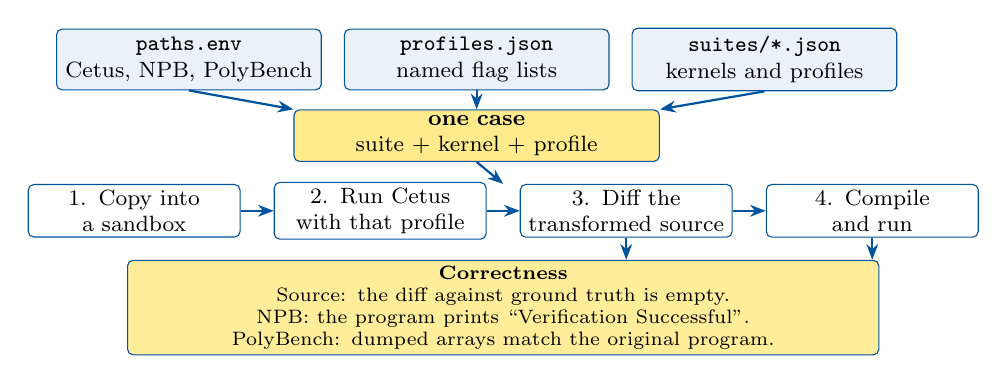
\begin{tikzpicture}[
      node distance=0.22cm and 0.28cm,
      cfg/.style={draw=udblue, rounded corners=2pt, fill=udblue!8,
                  align=center, inner sep=3pt, text width=3.15cm,
                  font=\footnotesize},
      word/.style={draw=udblue, rounded corners=2pt, fill=udgold!45,
                   align=center, inner sep=2pt, text width=4.5cm,
                   font=\footnotesize},
      stage/.style={draw=udblue, rounded corners=2pt, fill=white,
                    align=center, inner sep=2pt, text width=2.55cm,
                    font=\footnotesize},
      ok/.style={draw=udblue, rounded corners=2pt, fill=udgold!40,
                 align=center, inner sep=2pt, text width=9.4cm,
                 font=\scriptsize},
      arr/.style={-{Stealth[length=2mm]}, thick, udblue}
    ]
    \node[cfg] (env) {\texttt{paths.env}\\Cetus, NPB, PolyBench};
    \node[cfg, right=of env] (prof) {\texttt{profiles.json}\\named flag lists};
    \node[cfg, right=of prof] (suite) {\texttt{suites/*.json}\\kernels and profiles};
    \node[word, below=0.24cm of prof] (case) {\textbf{one case}\\suite + kernel + profile};
    \draw[arr] (env.south) -- (case.north west);
    \draw[arr] (prof) -- (case);
    \draw[arr] (suite.south) -- (case.north east);
    \node[stage, below=0.28cm of case, xshift=-4.35cm] (copy) {1. Copy into\\a sandbox};
    \node[stage, right=0.42cm of copy] (cetus) {2. Run Cetus\\with that profile};
    \node[stage, right=0.42cm of cetus] (diff) {3. Diff the\\transformed source};
    \node[stage, right=0.42cm of diff] (run) {4. Compile\\and run};
    \draw[arr] (copy) -- (cetus);
    \draw[arr] (cetus) -- (diff);
    \draw[arr] (diff) -- (run);
    \draw[arr] (case.south) -- ($(copy.north)!0.5!(run.north)$);
    \coordinate (rowmid) at ($(copy.south)!0.5!(run.south)$);
    \node[ok, below=0.28cm of diff.south -| rowmid, anchor=north] (check)
      {\textbf{Correctness}\\
       Source: the diff against ground truth is empty.\\
       NPB: the program prints ``Verification Successful''.\\
       PolyBench: dumped arrays match the original program.};
    \draw[arr] (diff.south) -- (diff.south |- check.north);
    \draw[arr] (run.south) -- (run.south |- check.north);
  \end{tikzpicture}

  \vspace{0.2em}
  \begin{minipage}{\linewidth}
  \raggedright\footnotesize
  A \textbf{kernel} is one program (\texttt{gemm}, \texttt{bt}).
  A \textbf{profile} is one named list of Cetus flags
  (\texttt{parallel}, \texttt{paw\_tiling\_nt}).
  A \textbf{benchmark} is that program taken from PolyBench or NPB.

  \vspace{0.35em}
  The JSON files in the diagram describe benchmark cases.
  Kernel snippets are JSON too, under \texttt{kernels/}.
  They stop after the source diff and are not compiled or run.
  \end{minipage}
  \note{Benchmark JSON is benchmarks/config/suites and profiles.json. Kernel snippets are benchmarks/config/kernels. Both load at runtime. The original NPB and PolyBench trees are never edited. Ground truth lives under ground\_truth/benchmarks/suite/profile/kernel. NPB verify looks for the verification-successful line. PolyBench diffs POLYBENCH\_DUMP\_ARRAYS output of the original and the transformed binary.}
\end{frame}

\begin{frame}{How a test is configured}
  A benchmark case is one triple from JSON: \textbf{suite}, \textbf{kernel}, \textbf{profile}.
  Kernel snippets are JSON suites too.
  Changing either file does not require rebuilding the harness.
  \vspace{0.45em}
  \begin{enumerate}
    \item Copy the kernel into a sandbox. The NPB and PolyBench trees stay untouched.
    \item Run Cetus with that profile's flags.
    \item Format the output and diff it against checked-in ground truth.
    \item Compile the transformed program and run it.
  \end{enumerate}
  \vspace{0.35em}
  \begin{tabular}{@{}lll@{}}
    \toprule
    Suite & Problem size & How the run is checked \\
    \midrule
    NPB 3.3 serial & class S & 4 threads, passive wait, verification string \\
    PolyBench/C 4.2 & MINI & 1 thread, dumped arrays match the original \\
    Kernel snippets & \texttt{kernels/*.json} & source diff only \\
    \bottomrule
  \end{tabular}\par
  \vspace{0.4em}
  Paths to Cetus, NPB, and PolyBench come from \texttt{paths.env}.
  \note{Say the JSON lives in benchmarks/config. Suites pick kernels, class or dataset, and which profiles apply. Profiles are a separate file of Cetus flags. Kernel snippets are benchmarks/config/kernels. Six unit-test programs check the harness itself and are not Cetus runs.}
\end{frame}

\begin{frame}{What is tested}
  \small
  \begin{tabular}{@{}llr@{}}
    \toprule
    Suite & Kernels & Count \\
    \midrule
    PAW tiling snippets & GEMM, 3mm, and four nest-shape cases & 6 \\
    Subscripted subscripts & AMG, EVSL, Gromacs, UA, and five others & 9 \\
    NPB serial & BT, SP, LU, MG, CG, FT, EP, IS, UA & 9 \\
    PolyBench & data mining, linear algebra, stencils, medley & 30 \\
    \bottomrule
  \end{tabular}\par
  \vspace{0.55em}
  Every profile starts from dependence analysis, privatization, reduction, and OpenMP output
  (\texttt{-ddt=2 -privatize=2 -reduction=2 -ompGen=1}).
  \vspace{0.35em}
  \begin{tabular}{@{}p{0.22\textwidth}p{0.22\textwidth}p{0.48\textwidth}@{}}
    \toprule
    Profile & Where & What is added \\
    \midrule
    parallel & NPB and PolyBench & OpenMP only. No tiling. \\
    paw\_tiling\_nt & NPB and PolyBench & PAW on. NT tile sizes, 4 cores, 25\,600\,KiB shared cache, 64-byte lines. \\
    paw\_tiling\_lrw & NPB and PolyBench & PAW on. LRW (FindB) tile sizes. Same cache model. \\
    paw\_tiling\_fixed32 & NPB and PolyBench & PAW on. Every tiled loop uses size 32. \\
    reuse\_analysis & NPB only & Reuse-vector analysis on. No tiling. \\
    \bottomrule
  \end{tabular}\par
  \note{Tiling snippets use the PAW flags, not these benchmark profiles. Subscript tests turn OpenMP generation off. The three PAW profiles differ only in tile-size selection. reuse\_analysis is NPB only because that is how the suite JSON is written. cacheSize is in kibibytes. The parallel profile is not stock Cetus: alias is 3 rather than 1, and profitable-omp is off.}
\end{frame}

\end{document}
